\documentclass[10pt,a4paper]{article}
\usepackage[utf8]{inputenc}
\usepackage{amsmath}
\usepackage{amsfonts}
\usepackage{amssymb}
\usepackage{graphicx}
\begin{document}
\section{Group Representations, Equivariance, and Invariance}
A group $G$ is a set with a binary, associative product defined between it's elements under which it is closed, and for which every element, there exists an inverse element (and which also contains an identity element). 

\subsubsection*{Matrix Representations of Groups}
A matrix representation $\mathcal{D}_{V}$ of a group $G$ is a map from elements of $G$ to square matrices such that for all elements $g,h\in G$, there are representations satisfying:
$$
\mathcal{D}(g)\mathcal{D}(h)=\mathcal{D}(gh)
$$
Note that we often discard the 'matrix' from 'matrix representation' and often refer only to representations of groups, though these are synonymous for our purposes here.


\subsubsection*{Equivariance}
A function $f:X\rightarrow Y$ is equivariant with respect to a group $G$ if, for representations $\mathcal{D}_X$ and $\mathcal{D}_Y$ of $G$ (over spaces $X$ and $Y$, respectively), it satisfies:
$$
f(D_X(g)x) = D_Y(g)f(x) \quad\quad \forall g\in G
$$
Essentially, a function is equivariant with respect to some group if it 'commutes' with the representations of groups on it's input and output space. 

\subsubsection*{Invariance}
A special case of equivariance then is \textit{invariance}, where the representations of all group elements in the output space are identity (i.e. $D_Y$ is the trivial representation). That is, a function $f:X\rightarrow Y$ is invariant under a group $G$ if it satisfies:
$$
f\circ \mathcal{D}_X(g) = f \quad
\ \forall g\in G.
$$

\section{Neural Networks}
Neural networks are a class of universal function approximators, composed layer-wise by functions $\mathcal{L}^1\circ\mathcal{L}^2\circ ... \circ \mathcal{L}^n $, where each layer-to-layer transition map $\mathcal{L}^i$ is a trainable function from some feature space associated with layer $L$ to a feature space associated with layer $L+1$.

\section{$SO(3)$ Equivariant Networks}
In the case of $SO(3)$, representations over a vector space of dimension $2\ell+1$ are Wigner-$\mathcal{D}^{\ell}$ matrices. Thus, we define an $SO(3)$ equivariant network to be a neural network $f:H_1 \rightarrow H_2$, with domain $H_1:\lbrace h_{(\ell_1)}\rbrace$ and codomain $H_2:\lbrace h'_{(\ell_2)}\rbrace$ (both being direct products of harmonic tensor spaces), that satisfies:
$$
f(\lbrace \mathcal{D}^{\ell_1}(R)h_{(\ell_1)}\rbrace) = \lbrace\mathcal{D}^{\ell_2}(R) h'_{(\ell_2)}\rbrace \quad\quad \forall R\in SO(3)
$$
The harmonic components $h_{\ell}^m$ (where $h_{\ell}$ generally refers to a $2\ell+1$ dimensional vector) correspond most naturally to the coefficients of spherical harmonic tensors, and in the context of machine learning, act as a feature space for data.

\subsection{Representation/Feature Space}
In an $SO(3)$-network, features are generally associated with irreducible representations of groups. In the case of $SO(3)$, these irreducible representations are spherical harmonics $Y_{\ell}^m$, indexed by two sets, the rotational order $\ell\geq 0$, and the azimuthal order $-\ell\leq m \leq \ell$.

Thus, a traditional feature set $V^{(n)a}$ of channel $a$ and associated with object $n$, has an additional two indices $\ell$ and $m$ in an $SO(3)$ network, corresponding to the aformentioned indices of a harmonic expansion.


\subsection{Layers}
Compositions of equivariant functions are themselves equivariant functions. As such, we may form an equivariant network by composing it layer-wise from a set of common equivariant functions.

Here, we consider three types of $SO(3)$-equivariant functions from which we may compose our equivariant networks: namely, $SO(3)$-feature convolutions, $\ell$-wise self-interactions and non-linearities, and pooling. An overview of each is given below.

\subsubsection{$SO(3)$ Convolution}
To maintain equivariance, for an input feature set of the type described above,  through convolution with some filter $F$,  the filter also must be associated with a set of spherical harmonics, and thus also has an additional two indices $\ell_f$ and $m_f$. 

Note here that the tensor product of two representation spaces is equivariant under transformation of the two subspaces, i.e.:
$$
\mathcal{D}^V\otimes \mathcal{D}^W=\mathcal{D}^{V\otimes W}
$$
Tensors products of $SO(3)$ representations are cleanly related to a third set of $SO(3)$ representations by way of Clebsch-Gordan coefficients $c^{\ell_3m_3}_{\ell_1m_1\ell_2m_2}$ as:
$$
(u\otimes v)_{\ell_o}^{m_o} = c_{\ell_1m_1\ell_2m_2}^{\ell_om_o}u_{\ell_1}^{m_1}v_{\ell_2}^{m_2}
$$
where $u$ and $v$ are harmonic vectors of order $\ell_1$ and $\ell_2$, respectively.

Thus, we maintain equivariance by defining convolution to be the scaled tensor product of the two representation spaces (i.e. that of the input feature space, and the filter space), so that layer to layer convolutional maps $\mathcal{L}$ may be defined component-wise as:
$$
\mathcal{L}^{\ell_o}_{acm_o}\big(\vec{r}_a,V_{acm_i}^{\ell_i}\big) = \sum_{m_f,m_i}c_{\ell_im_i\ell_fm_f}^{\ell_o m_o}\sum_{b}F^{\ell_f\ell_i}_{cm_f}(r_{ab})V_{bcm_i}^{\ell_i}
$$
where the filter function $F^{\ell_f\ell_i}_{cm_f}(r_{ab})$ depends only on the distance between point $a$ and $b$ (as opposed to directional dependence, to maintain equivariance), but has independent, trainable parameters for different rotational orders $\ell_f, \ell_i$, azimuthal orders $m$, and channels $c$.

\subsubsection{Self-Interaction}
Feature sets for individual objects may also update according to themselves as long as they act across $m$ for every $\ell$ and only update accordign to the different channels $c$. That is, functions of the form:
$$
V_{acm}^{\ell} \rightarrow  \sum _{c}W^{\ell}_{c'c}V_{acm}^{\ell}
$$
are also equivariant. 

\subsubsection{Non-Linearities}
We can also apply point-wise non linearities and maintain equivariance, as long as they also act across $m$ indices for every order feature $\ell$.

\subsubsection{Pooling}
Pooling, or aggregation, across all elements or objects (index $a$) while preserving the $m$ and $\ell$ indices is itself equivariant. Thus, functions of the form:
$$
 M_{cm}^{\ell} = \text{AGG}_{a}(\lbrace V_{acm}^{\ell}\rbrace)
$$ 
where $\text{AGG}$ is an arbitrary aggregation function performed only over the object index $a$, are also available in the construction of $SO(3)$ networks.

\subsection{Predicting Tensorial Data with SO(3) Networks}
Such $SO(3)$ equivariant networks are naturally well suited for the prediction of tensorial properties. Tensors may generally be decomposed into a set of $SO(3)$ invariant subspaces which can then each be associated with a set of spherical harmonics (see spherical harmonic decomposition of a tensor).

\subsubsection{Feature Pathways}
It should be clear that, from our definition of $SO(3)$ equivariant convolution, different order $\ell$ representations in the output space $V^{(L), \ell}_{acm}$ of final layer $L$, will be the result of interactions with potentially different $\ell_f$ order filters and the input layer features of order $\ell_i$. We here term the set of filter orders through the layers that result in a final output feature of order $\ell_o$ to be the \textit{feature pathway} of feature order $\ell_o$.

This feature pathway depends most generally on the chosen input feature orders $\ell_i$, as well as the order of the filters  $\ell_f$ for each layer, and the total number of layers. The pathway then may be determined by the selection rules of Clebsch-Gordon coefficients. That is, CG coefficients $c^{LM}_{\ell_1m_2\ell_2m_2}$ can only be non-zero when the following hold for some set of inputs $\ell_1,m_1$ and $\ell_2, m_2$:
\begin{itemize}
\item $M=m_1+m_2$
\item $|\ell_1-\ell_2|\leq L\leq \ell_1+\ell_2$
\end{itemize}
Thus, we may determine what filter orders $\ell_f$ contribute to some output of order $\ell_o$ of some network, for an input of order $\ell_i$.

Feature pathways are particularly relevant in the case of tensorial multi-target training sets, or transfer-learning applications, where different targets have different rotational order decompositions. In such cases, the filters learned for different datasets may not overlap at all, and thus would have disjoint feature pathways. 

For example, consider one layer of $SO(3)$ convolution, with input features of order $\ell_i=0,1$ and filters of order $\ell_f = 0,1,2$. The outputs of order $\ell_{o}=1$ would depend only on the trained parameters in filters of orders $\ell_i,\ell_f = (0,1),(1,0)$, whereas the outputs of order $\ell_{o}=2$ would depend only on filters of $\ell_i,\ell_f = (0,2),(1,1)$. 
\begin{center}
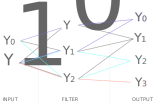
\includegraphics[scale=0.5]{featurepath_ex_12.pdf}
\end{center}
So, if a network was trained on a tensorial target set with a decomposition of order $\ell_o=2$ (i.e. a rank-two symmetric, traceless tensor), and then transfered and trained on a tensorial target of order $\ell_o = 3$ (i.e. a symmetric, traceless rank-3 tensor), there would only be overlap in the training of the $\ell_f=1$ filter weights.




\end{document}